% Two probabilistic routes with the original exact teaching values.
% Volume three architecture figures. Independent export only; not book fonts.
\colorlet{MutedBlueFill}{FigureBlueFill}
\colorlet{MutedGreenFill}{FigureGreenFill}
\colorlet{MutedPurple}{FigurePurple}
\colorlet{MutedPurpleFill}{FigurePurpleFill}
\tikzset{
 v3 picture/.style={x=1mm,y=1mm,font=\figurefont\fontsize{8}{10}\selectfont,text=FigureInk,line width=.65pt},
 v3 box/.style={draw=FigureBlue,fill=white,rounded corners=1.8pt,line width=.7pt,inner sep=2.5pt,align=center},
 v3 data/.style={v3 box,fill=FigureBlueFill},
 v3 model/.style={v3 box,draw=FigureGreen,fill=FigureGreenFill},
 v3 output/.style={v3 box,draw=FigureYellow,fill=FigureYellowFill},
 v3 risk/.style={v3 box,draw=FigureRed,fill=FigureRedFill},
 v3 group/.style={draw=FigureBlue,rounded corners=1.8pt,line width=.65pt,inner sep=3mm},
 v3 flow/.style={draw=FigureStroke,line width=.75pt,-{Stealth[length=1.65mm,width=1.05mm]},rounded corners=1pt},
 v3 guide/.style={draw=FigureMuted,line width=.6pt,dashed},
 v3 feedback/.style={v3 flow,draw=FigureGreen,dashed},
 v3 title/.style={draw=none,fill=none,font=\figurefont\fontsize{8}{10}\selectfont,align=center,inner sep=1pt},
 v3 note/.style={draw=none,fill=none,font=\FigureNoteFont\fontsize{7.5}{9.5}\selectfont,text=FigureMuted,align=center,inner sep=1pt},
 v3 label/.style={draw=none,fill=none,font=\figurefont\fontsize{8}{10}\selectfont,align=center,inner sep=1pt},
 v3 wire/.style={draw=FigureMuted,line width=.45pt},
 v3 point/.style={circle,draw=FigureBlue,fill=FigureBlueFill,minimum size=2.3mm,inner sep=0pt,line width=.55pt}
}
% Bring pre-existing native TikZ geometry to the same typography and scale.
\tikzset{
 foundation picture/.append style={font=\figurefont\fontsize{8}{10}\selectfont,line width=.65pt},
 foundation node/.append style={rounded corners=1.8pt,line width=.7pt,font=\figurefont\fontsize{8}{10}\selectfont},
 foundation heading/.append style={draw=none,fill=none,font=\figurefont\fontsize{8}{10}\selectfont},
 foundation note/.append style={draw=none,fill=none,font=\FigureNoteFont\fontsize{7.5}{9.5}\selectfont},
 foundation flow/.append style={line width=.75pt,-{Stealth[length=1.65mm,width=1.05mm]}},
 foundation frame/.append style={rounded corners=1.8pt,line width=.7pt},
 foundation edge label/.append style={draw=none,fill=none,font=\figurefont\fontsize{8}{10}\selectfont}
}
% Official Lucide outline icons, consistently used across diagrams. Size in mm.
\newcommand{\VIcon}[5]{\node[inner sep=0pt] at (#2,#3) {\includegraphics[width=#4mm]{figures/03-foundations/00-shared/tikz/icons/#1-#5.pdf}};}
% A neutral network glyph (not a claim about an actual model architecture).
% Coordinates denote its centre; scale 1 gives 13 x 8 mm.
\newcommand{\VNet}[4]{\begin{scope}[shift={(#1,#2)},scale=#3]
 \foreach \a in {-3,0,3}{\foreach \b in {-3,0,3}{\draw[v3 wire] (-5,\a)--(0,\b);}}
 \foreach \a in {-3,0,3}{\draw[v3 wire] (0,\a)--(5,0);}
 \foreach \a in {-3,0,3}{\draw[draw=#4,fill=#4,line width=.55pt] (-5,\a) circle(.9);\draw[draw=#4,fill=white,line width=.55pt] (0,\a) circle(.9);}
 \draw[draw=#4,fill=#4,line width=.55pt] (5,0) circle(.9);
\end{scope}}
\newcommand{\VDots}[4]{\foreach \k in {0,1,2,3}{\fill[#4] ({#1+2.7*\k},#2) circle(#3);}}
% Feature vector/tensor elements are scientific glyphs, not decorative icons.
\newcommand{\VVector}[4]{\foreach \k in {0,...,4}{\fill[#4,rounded corners=.25pt] ({#1+2.2*\k},#2) rectangle ++(1.5,#3);}}

\tikzset{v3 flow/.append style={line width=.95pt,rounded corners=1.8pt},v3 box/.append style={line width=.85pt}}
\newcommand{\DGMail}[4]{\VEnvelope{#1}{#2}{.55}{#3}\ifnum#4=1\draw[draw=#3,fill=white,line width=.75pt] (#1+2.8,#2-1.6) circle(1.65);\draw[draw=#3,line width=.9pt] (#1+1.6,#2-.4)--(#1+4,#2-2.8);\fi}
\begin{tikzpicture}[v3 picture]
\path[use as bounding box] (0,0) rectangle (163,125);
\draw[draw=FigureBlue,fill=white,rounded corners=.7pt,line width=.9pt] (1,76.5)--(15,76.5)--(15,90.5)--(12,94)--(1,94)--cycle;
\draw[draw=FigureBlue,fill=FigureBlueFill,line width=.7pt] (12,94)--(12,90.5)--(15,90.5);
\VEnvelope{7}{88}{.62}{FigureBlue}\foreach \y in {83,80.5}{\draw[draw=FigureBlue,line width=1.15pt,line cap=round] (3,\y)--(12,\y);}
\node[v3 label] at (8,73.5) {邮件};
\draw[v3 box] (19,77) rectangle (24,95);
\foreach \y in {80,84,88,92}{\fill[FigureBlue] (21.5,\y) circle(.8);}
\node[v3 label] at (21.5,73) {特征 $x$};
\draw[v3 flow] (14,85)--(19,85);
\node[v3 title] at (78,120) {判别式：直接估计条件概率};
\node[v3 data,minimum width=27mm,minimum height=17mm] (disc) at (53,106) {};
{\colorlet{VNetworkInput}{FigureBlue}\colorlet{VNetworkHidden}{FigureBlue}\colorlet{VNetworkOutput}{FigureBlue}\VLayerNet{53}{103}{1.1}{3}{3}{1}}
\node[v3 label] at (53,112) {得分 $s=\ln 3$};
\node[v3 box,draw=FigurePurple,minimum width=22mm,minimum height=16mm] (sig) at (86,106) {};
\node[v3 label] at (86,111) {$\sigma(s)$};
\draw[draw=FigurePurple,line width=1.05pt] (81,102)..controls(87,101)and(85,108)..(91,107);
\draw[v3 flow] (24,85)--(31,85)|-(disc.west);
\draw[v3 flow] (disc.east)--(sig.west);
\node[v3 title] at (142,120) {类别后验};
\node[v3 box,minimum width=29mm,minimum height=8mm] (p0) at (142,112) {};
\node[v3 box,draw=FigureGreen,minimum width=29mm,minimum height=8mm] (p1) at (142,99) {};
\DGMail{133}{112}{FigureBlue}{0}\node[v3 label] at (147,112) {$0.25$};
\DGMail{133}{99}{FigureGreen}{1}\node[v3 label] at (147,99) {$0.75$};
\draw[v3 flow] (sig.east)--(108,106)|-(p0.west);
\draw[v3 flow,draw=FigureGreen] (sig.east)--(108,106)|-(p1.west);
\node[v3 title] at (80,88) {生成式：联合概率再归一化};
\foreach \y/\i/\a/\b/\c in {77/0/0.8/0.01/FigureBlue,61/1/0.2/0.12/FigureGreen}{
 \node[v3 box,draw=\c,minimum width=19mm,minimum height=11mm] (prior\i) at (46,\y) {};
 \node[v3 label] at (46,\y+3.2) {$p(y=\i)$};\DGMail{41}{\y-2}{\c}{\i}\node[v3 label] at (50,\y-2) {$\a$};
 \node[v3 box,draw=\c,minimum width=24mm,minimum height=11mm] (like\i) at (75,\y) {};
 \node[v3 label] at (75,\y+3.2) {$p(x\mid y=\i)$};\VDocument{67.5}{\y-2}{.45}{\c}\node[v3 label] at (78,\y-2) {$\b$};
 \node[circle,draw=\c,minimum size=5mm,inner sep=0pt] (mul\i) at (96,\y) {$\times$};
 \draw[v3 flow] (31,85)|-(prior\i.west);
 \draw[v3 flow] (prior\i.east)--(like\i.west);
 \draw[v3 flow] (like\i.east)--(mul\i.west);
}
\node[v3 note] at (96,83) {$0.008$};\node[v3 note] at (96,67) {$0.024$};
\node[v3 box,draw=FigureYellow,minimum width=17mm,minimum height=14mm] (norm) at (117,69) {};
\fill[FigureRed] (117,69) circle(3.7);\node[font=\figurefont\fontsize{12}{12}\selectfont,text=white] at (117,69.1) {$\div$};
\node[v3 label] at (117,80) {归一化};\node[v3 note] at (117,58) {除以 $0.032$};
\draw[v3 flow] (mul0.east)--(104,77)|-(norm.west);
\draw[v3 flow] (mul1.east)--(104,61)|-(norm.west);
\node[v3 title] at (145,85) {类别后验};
\node[v3 box,minimum width=27mm,minimum height=8mm] (q0) at (145,76) {};
\node[v3 box,draw=FigureGreen,minimum width=27mm,minimum height=8mm] (q1) at (145,62) {};
\DGMail{136.5}{76}{FigureBlue}{0}\node[v3 label] at (150,76) {$0.25$};
\DGMail{136.5}{62}{FigureGreen}{1}\node[v3 label] at (150,62) {$0.75$};
\draw[v3 flow] (norm.east)--(127,69)|-(q0.west);
\draw[v3 flow,draw=FigureGreen] (norm.east)--(127,69)|-(q1.west);
% Analytical vector panels are retained from the corresponding Matplotlib source.
\node[v3 title] at (40,52) {条件类别概率};
\node[v3 title] at (121.5,52) {先验加权的联合密度};
\node[inner sep=0pt,anchor=south west] at (7,0) {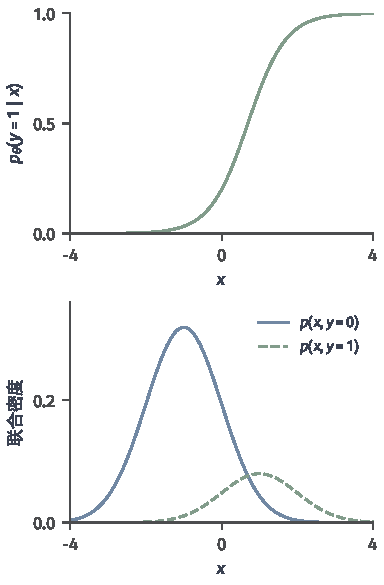
\includegraphics[width=65mm,trim=0 140.315pt 0 0,clip]{figures/03-foundations/01-basics/tikz/models-discriminative-generative/assets/probability-panels.pdf}};
\node[inner sep=0pt,anchor=south west] at (89,0) {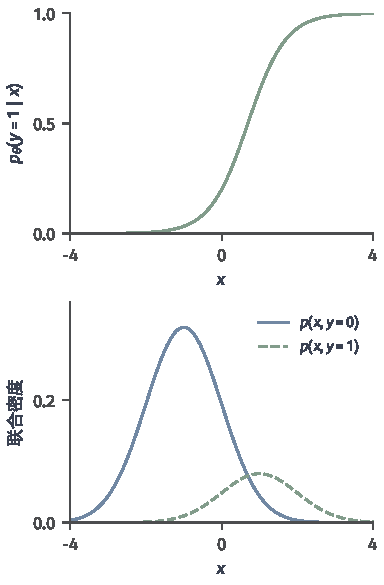
\includegraphics[width=65mm,trim=0 0 0 140.315pt,clip]{figures/03-foundations/01-basics/tikz/models-discriminative-generative/assets/probability-panels.pdf}};
\end{tikzpicture}
